\documentclass[conference]{IEEEtran}

% ---------------------------------------------------------
% PACKAGES
% ---------------------------------------------------------

\usepackage{amsmath, amssymb}
\usepackage{graphicx}
\usepackage{booktabs}
\usepackage{multirow}
\usepackage{url}
\usepackage{hyperref}
\usepackage{enumitem}
\usepackage{float}
\usepackage{array}
\usepackage{cite}
\usepackage{xcolor}
\definecolor{sectionblue}{RGB}{0,51,102}

% ---------------------------------------------------------
% HYPERLINK SETUP
% ---------------------------------------------------------

\hypersetup{
    colorlinks=true,
    linkcolor=black,
    citecolor=black,
    urlcolor=blue
}

% ---------------------------------------------------------
% DOCUMENT
% ---------------------------------------------------------

\begin{document}
\pagestyle{plain}

% ---------------------------------------------------------
% TITLE
% ---------------------------------------------------------

\title{
    PACE: Patch-Adaptive Cross-Attention for Efficient Multimodal Sensor Fusion
    \\
    \vspace{0.5em} \large \emph{Research Proposal}
}

\author{
    \IEEEauthorblockN{Tegan Hakim, Gili Gordiyenko}
    \IEEEauthorblockA{
        Department of Computer Science\\
        University of Maryland, College Park\\
        College Park, MD, USA\\
        September 2026
    }
}

\maketitle

% =========================================================
% 1. BACKGROUND
% =========================================================
\color{black}
\section{Background}
\color{black}

\subsection{Problem Definition and Importance}
Visible/RGB and Infrared (IR) imaging are critical sensing modalities that power modern computer vision systems, particularly those in military contexts. Visible/RGB and IR are the backbone of defense-focused operations, including but not limited to intelligence, surveillance, and reconnaissance (ISR), target tracking, and domain awareness. Unmanned Aerial Vehicles (UAVs) increasingly serve as the primary platforms through which these missions are executed, providing persistent sensing capabilities in contested operational environments. However, UAVs face the critical challenge of operating under limited system resources and frequently in sensor-degrading environments such as adverse weather, sensor noise, and occlusion. Consequently, the quality of RGB data is often compromised, which severely reduces operational confidence and mission efficacy. For this work, we consider a UAV-based ISR use case focused on the detection of ground vehicles to support situational awareness and intelligence collection.

IR sensors can reliably collect data in environmental conditions where RGB is unpredictable. Multimodal fusion can improve perception by leveraging complementary information when one modality is degraded. Recent approaches implement multimodal fusion for hybrid imaging and dynamically weight modalities based on local features. However, existing approaches perform fusion without regard for existing modality reliability, potentially incurring unnecessary computation on regions where additional cross-modal information provides limited benefit. Low-SWaP (size, weight, and power) systems such as UAVs have resource constraints including limited latency, memory, and processing power, making this unnecessary overhead especially costly. PACE addresses this inefficiency by selectively applying patch-level cross-attention based on modality reliability through a learned, system-aware gating mechanism, allocating computational resources where cross-modal information is most valuable.


\subsection{Research Question}

\begin{quote}
\textit{Can reliability-gated, patch-level cross-attention reduce inference cost and latency relative to dense multimodal fusion while preserving detection accuracy under low-SWaP edge constraints? 
}
\end{quote}

% =========================================================
% 2. LITERATURE REVIEW
% =========================================================
\color{black}
\section{Literature Review}
\color{black}

\subsection{Multimodal Visible--Infrared Fusion}

FusionNet introduces a modality-aware framework that dynamically weights infrared and visible features across spatial regions to perform infrared and visible image fusion (IVIF) \cite{fusionnet2025}. Through this mechanism, relative informativeness of infrared and visible features determine their respective influence on the final image \cite{fusionnet2025}. This amplification of task-critical regions, combined with pixel-wise alpha blending, achieves high-quality multimodal fusion \cite{fusionnet2025}. \

\indent FusionNet uses separate encoders for IR and visual information, and a learned alpha blending module to adaptively combine information from both sensors \cite{fusionnet2025}. The framework achieves strong fusion quality, preserving critical infrared information and visible scene details \cite{fusionnet2025}. However, FusionNet performs fusion computation across the entire image, disregarding areas of high visible image quality where computation may be excessive. PACE extends this idea by using patch-level reliability estimates to determine where fusion is beneficial.

\subsection{CrossFuse}

CrossFuse is an infrared-visible image fusion model that emphasizes less-correlated features between inputs to combine complementary information from both modalities \cite{crossfuse2024}. The framework involves separate encoders for IR and visible inputs, self-attention, cross-attention, and a decoder that reconstructs the fused image \cite{crossfuse2024}. Training consists of two phases, first pretraining the modality-specific autoencoders and then the fusion model training \cite{crossfuse2024}. CrossFuse uses reverse softmax to emphasize low-similarity features so information unique to each modality is preserved \cite{crossfuse2024}. \

\indent
CrossFuse demonstrates that cross-attention is effective for multimodal fusion, achieving strong preservation of infrared and visible image features \cite{crossfuse2024}. A key limitation of the approach is that fusion computation is still applied broadly to the whole image rather than on focused areas. The model's dense cross-attention computations represent the primary computational cost that PACE aims to reduce through local reliability estimation and dynamic cross-attention execution, therefore forming a solid baseline. PACE extends CrossFuse by shifting from dense, full-image fusion toward reliability-guided, selective cross-attention designed to improve efficiency under low-SWaP constraints.

% =========================================================
% 3. PROJECT GOALS
% =========================================================
\color{black}
\section{Project Goals}
\color{black}

\begin{enumerate}
    \item Reproduce a dense CrossFuse-based multimodal fusion baseline modified to produce object detections.
    \item Develop a patch-level visible/IR quality and reliability estimation model. 
    \item Design and train a lightweight learned gating model to determine which patches require cross-attention. 
    \item Implement the overall PACE framework to produce object detections.
    \item Evaluate PACE against appropriate baselines under varying resource constraints using detection accuracy, inference latency, and computational cost. 
\end{enumerate}

% =========================================================
% 4. PROPOSED APPROACH
% =========================================================

\section{Proposed Approach}

\subsection{System Architecture}

\begin{figure}[H]
    \centering
    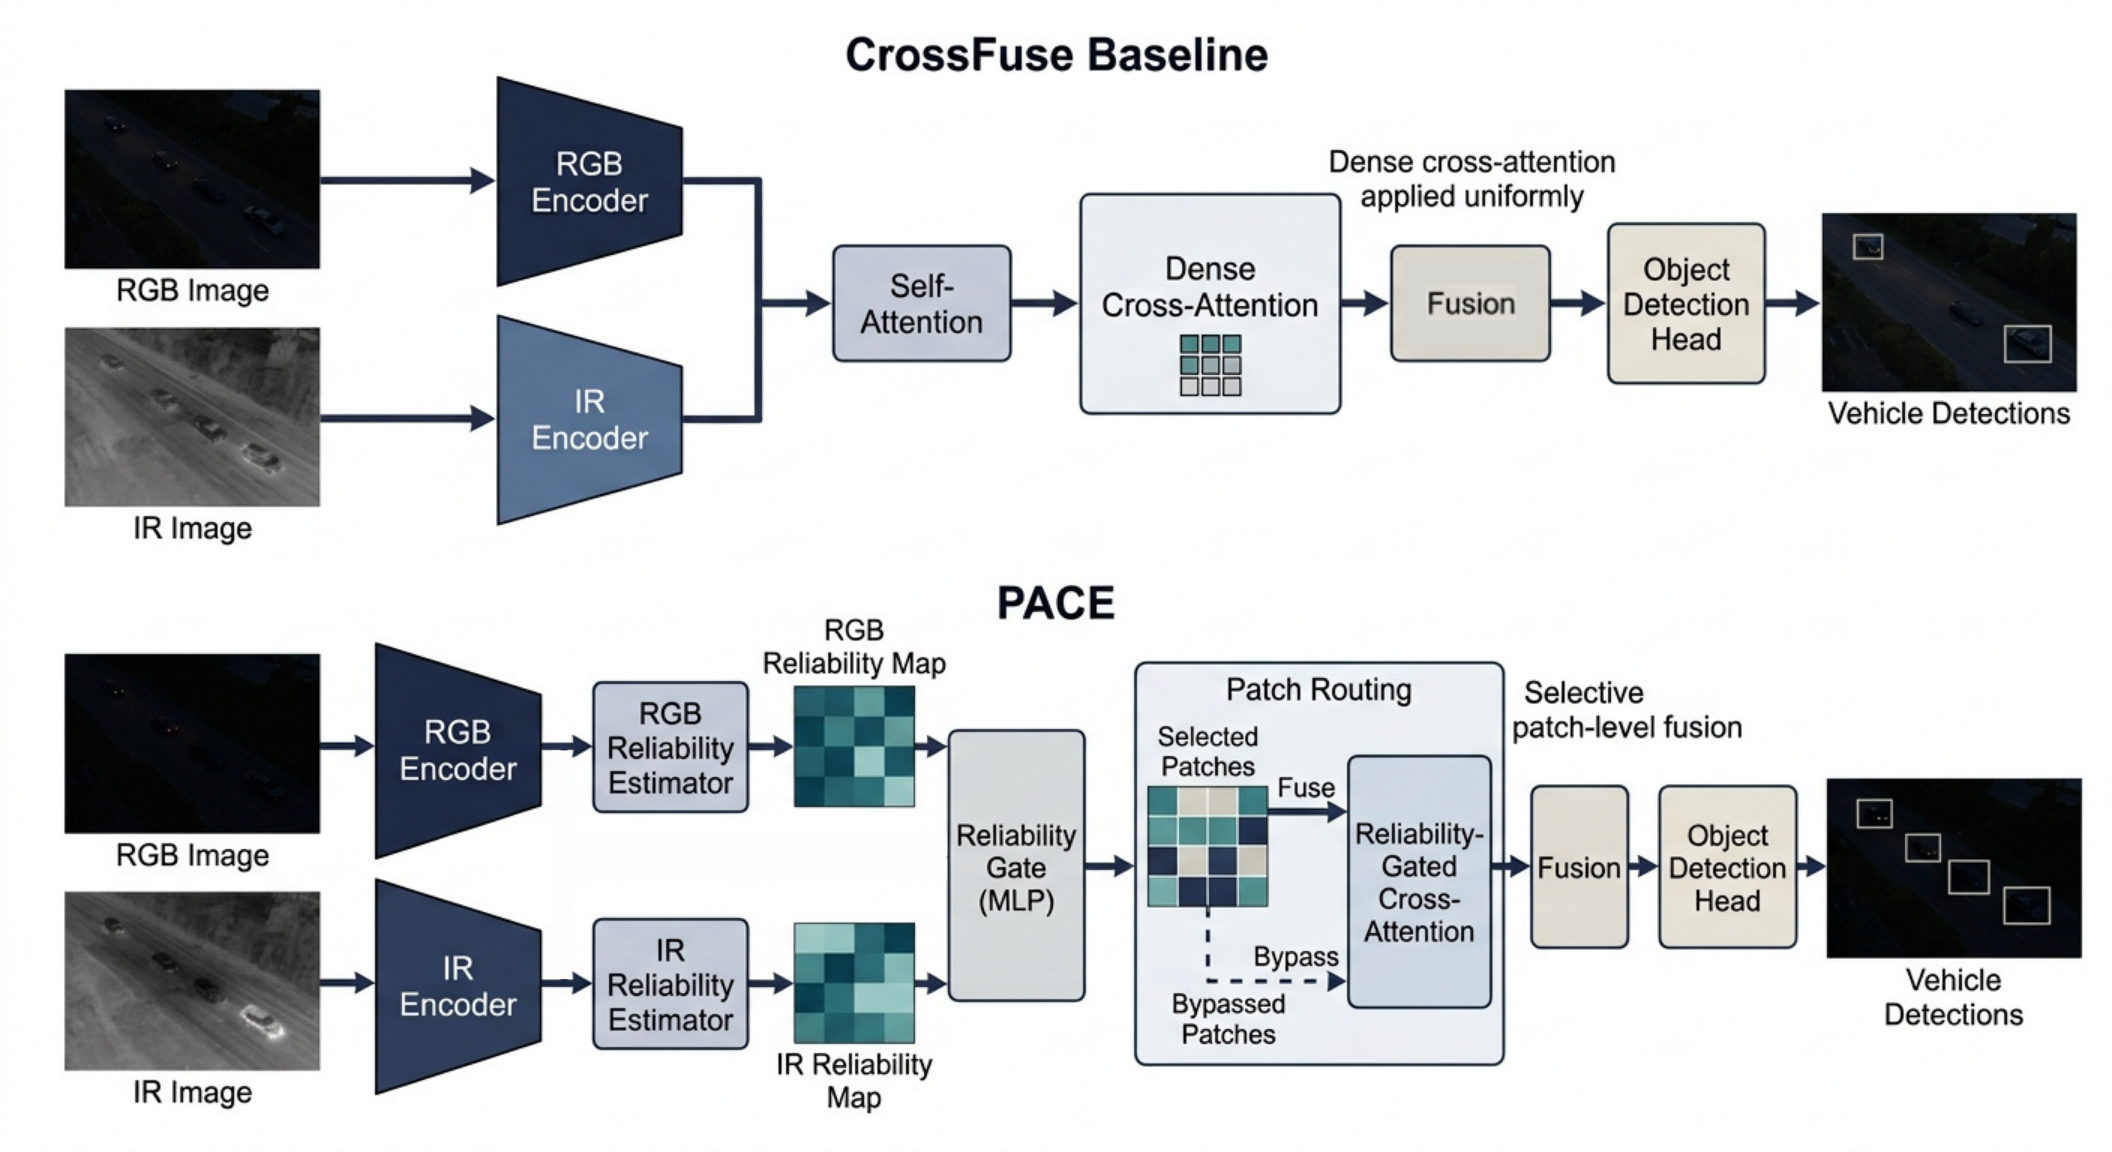
\includegraphics[width=\columnwidth]{architecture_comparison.png}
    \caption{Proposed PACE architecture.}
    \label{fig:architecture}
\end{figure}

The architecture for PACE begins with one encoder for each modality to perform feature extraction and embedding.
A learned patch reliability estimator then computes a quality score for each patch within the Visible/RGB and IR images. Two parallel 
estimators will be trained, one for each modality. A reliability gate model then determines which patches require fusion, taking into account
the quality scores of both modalities as well as Low-SWaP system and environmental considerations. 

\subsection{Feature Extraction}

PACE adopts the CrossFuse feature-extraction backbone, which uses separate convolutional encoders for visible/RGB and infrared inputs to learn modality-specific spatial features. Each encoder captures low-level texture information and higher-level semantic features while preserving corresponding spatial locations and compatible feature-map dimensions across modalities, enabling effective multimodal fusion.

\subsection{Patch-Level Quality / Reliability Estimation}

PACE introduces separate reliability estimation models for the RGB and IR modalities. Each input image is divided into a grid of patches, and the corresponding estimator predicts a reliability score for each patch. These scores are then normalized, with a high score indicating high trust in the data and strong reliability for downstream tasks such as object detection, while a low score indicating degradation caused by factors such as fog, limited light, or sensor damage. The estimators will be trained using human-labeled quality scores for image patches exhibiting realistic low-light conditions and other forms of degradation, and if time permits, synthetically degraded images with known degradation levels as well. The resulting patch-level reliability scores for each modality are provided to the reliability gate, which determines where cross-modal fusion is most beneficial.

\subsection{Reliability-Gated Cross-Attention}

While the baseline approach performs cross attention on the entire image, PACE uses a lightweight multilayer perceptron (MLP) to determine where fusion is effective. For each patch, the MLP takes into consideration the reliability scores of both modalities and current system resource levels. The MLP outputs a binary decision indicating whether fusion should be performed for the patch. Patches for which additional cross-modal information provides limited benefit can bypass the computationally expensive fusion operation, preserving resources for patches where fusion is more valuable. This selective routing enables PACE to leverage complementary information across modalities while reducing unnecessary cross-attention computation in regions where it provides limited benefit.

\subsection{Training Procedure}

The first phase of training will be reproducing the CrossFuse baseline, adding on an object-detection head, and training it on the DroneVehicle annotated datatset \cite{dronevehicle}. The reliability estimators for RGB and IR modalities will be trained using paired image patches and their corresponding quality information. Then, the multilayer perceptron gating model will learn a routing policy using the resulting reliability scores and resource constraints. Following the end-to-end PACE pipeline buildout and evaluation, additional fine-tuning may be performed, if time permits, to improve coordination among the reliability estimators, gating model, and object detection model. 

% =========================================================
% 5. EVALUATION
% =========================================================

\section{Evaluation / Success Criteria}

PACE will be evaluated by comparing its detection performance and computational efficiency against the modified CrossFuse baseline. Detection performance will be measured using precision, recall, F1-score, and mean Average Precision (mAP). Computational efficiency will be evaluated using inference latency and frames per second (FPS), along with GPU utilization and memory usage during inference. The primary objective is to determine whether PACE can reduce computational and latency requirements relative to dense cross-attention while maintaining comparable object detection performance.

% =========================================================
% 6. HARDWARE AND SOFTWARE
% =========================================================
\color{black}
\section{Hardware and Software Platform}
\color{black}

\subsection{Software}

PACE will be implemented in Python using the PyTorch library for model development and training. Libraries such as NumPy, Pandas, and OpenCV will also be used for tasks such as data preprocessing and manipulation. Additional libraries will be integrated as needed for visualization, pipeline performance tracking, etc. 

\subsection{Hardware}

This effort will require access to an NVIDIA CUDA-capable GPU through a provided virtual machine. GPU acceleration will be used to train the CrossFuse baseline as well as the proposed PACE architecture, including the feature encoders, reliability estimation models, gated cross-attention models, and detection head.

While Low-SWaP devices are known to use architectures such as the Jetson Orin series, we do not have access to such hardware. Instead, we will keep the system hardware and architecture fixed while measuring the differences between our outlined evaluation criteria. While this may not directly measure edge device performance, it provides a controlled experiment to determine whether the differences between PACE and the CrossFuse baseline produce significant findings.


% =========================================================
% 7. DATASETS
% =========================================================

\section{Datasets}

For this project, we will be using the VisDrone-DroneVehicle dataset, a large aerial RGB-IR vehicle detection dataset. The dataset consists of 56,878 total individual images which form 28,439 corresponding RGB-IR pairs. These images were captured from drone footage of parking lots, urban/resedential areas, and other environments, and include data from daytime and nighttime conditions. The RGB and IR image pairs are aligned and complete with bounding-box annotations for five vehicle categories: car, truck, bus, van, and freight\_car \cite{dronevehicle}. The dataset is already divided into training, validation, and test sets with 17,990, 1,469, and 8,980 pairs each\cite{dronevehicle}.

DroneVehicle is the right fit for PACE as it contains aligned IR and RGB data, as well as the environmental variation necessary to evaluate reliability-guided multimodal fusion. In a Low-SWaP UAV ISR scenario, a vehicle-detection system may make a sensing observation where certain regions are more robust in their RGB quality, and others where the IR modality provides more useful information. Instead of blindly applying the computationally expensive cross-attention fusion to the entire image, PACE will use patch-specific reliability estimates to identify where cross-modal information adds the most value. 

The dataset will be used to train both the modified CrossFuse baseline and the proposed PACE architecture with the same preprocessing, splits, and image pairings for both. RGB and IR pairs will be loaded together and passed through their respective feature encoders. The training set will be used for model training, the validation set will be used for tuning hyperparameters, and the test set will be saved for final evaluation between the CrossFuse baseline and PACE.

If time allows, we will expand our dataset by applying controlled synthetic degradations during training and evaluation. These degradations may include poor illumination levels, blur, noise, and other impairments that simulate conditions that reduce sensor reliability. This will enable evaluation of whether PACE can identify degraded regions and increase reliance on complementary modality information while avoiding unnecessary fusion computation in regions where the alternate modality remains reliable. 

All experiments will use identical dataset splits and preprocessing steps for the CrossFuse baseline and PACE to ensure that observed differences in detection performance and computational cost can be solely attributed to the proposed architecture rather than side-effects from inconsistencies in the training data.

The dataset is publicly available through Kaggle\footnote{\url{https://www.kaggle.com/datasets/brendanalvey/visdrone-dronevehicle}}.

% =========================================================
% 8. VALIDATION AND TESTING
% =========================================================

\section{Validation and Testing}

\subsection{Unit Tests}

Each major component of the PACE framework will have corresponding unit tests to verify tensor dimensions, numerical validity, and expected component behavior.

\renewcommand{\arraystretch}{1.15}
\begin{table}[H]
\centering
\caption{Planned Unit Tests}
\label{tab:tests}
\begin{tabular}{p{0.25\columnwidth} p{0.65\columnwidth}}
\toprule
\textbf{Component} & \textbf{Planned Test} \\
\midrule
Data loader & Verify paired RGB-IR images and ground-truth labels have expected dimensions and correspondence. \\
Preprocessing & Verify consistent resizing, normalization, and modality-specific transformations. \\
Feature extractor & Verify expected feature-map dimensions at each encoder stage. \\
Quality estimator & Verify patch-level reliability maps have expected dimensions and bounded values. \\
Attention & Verify reliability-weighted attention preserves expected tensor dimensions and produces finite outputs. \\
Fusion module & Verify RGB and IR features are spatially aligned before fusion. \\
Loss functions & Verify finite loss values and valid gradient propagation. \\
Inference & Verify complete RGB-to-IR fusion and detection pipeline executes successfully. \\
\bottomrule
\end{tabular}
\end{table}

% =========================================================
% 9. HUMAN EFFORT
% =========================================================

\section{Human Effort and Research Contribution}

While agentic artificial intelligence (AI) tools can be used to accelerate the implementation of proposed software such as the PACE pipeline, there exists a human factor that can't quite be replicated by modern-day models. Agentic AI systems cannot independently replace the human judgment and intuition required to define the PACE framework itself. For example, the quality estimation model is a central component of PACE, and although an agent can assist with its code implementation, defining which image features are low vs. high quality requires human domain knowledge and judgment. Model training is also a very manual process that involves dataset collection, data pre-processing, data labeling, and then the train/validation/evaluation loop. Human contribution is also necessary to configure the development environment, ensure proper testing frameworks, control the data-flow pipeline, select appropriate evaluation criteria, as well as determine whether experimental results are meaningful within the intended operational context. Therefore, agentic AI will take on the role of a technical aid to speed up development during the project rather than a substitute for the human-driven research decisions that define the system and its objectives.

% =========================================================
% 10. DOCUMENTATION AND DISTRIBUTION
% =========================================================

\section{Documentation and Distribution}

The PACE framework will be maintained in a public GitHub repository to support transparency, reproducibility, and future development. The repository will contain the baseline implementation of the CrossFuse architecture, proposed PACE architecture, documentation, experiment reports, and supporting code. The planned repository structure is as follows:

\begin{table}[H]
\centering
\caption{Planned GitHub Repository Structure}
\label{tab:repository}
\renewcommand{\arraystretch}{1.15}
\begin{tabular}{p{0.28\columnwidth}p{0.62\columnwidth}}
\toprule
\textbf{Path} & \textbf{Purpose} \\
\midrule
\texttt{baseline/} & Modified CrossFuse implementation with an object detection head for baseline comparison. \\

\texttt{pace/} & PACE architecture and implementation. \\

\texttt{reports/} & Project proposal, final paper, and supporting documentation. \\

\texttt{tests/} & Unit tests for major system components. \\

\texttt{README.md} & Installation, dataset preparation, training, evaluation, and experiment reproduction instructions. \\

\texttt{requirements.txt} & Required Python packages and dependencies. \\

\textit{Additional files} & Configuration files, experiment scripts, and other supporting resources. \\
\bottomrule
\end{tabular}
\end{table}

The repository documentation will provide instructions for reproducing the experimental pipeline from environment setup through evaluation. Specifically, the \texttt{README.md} will document installation and setup, dataset processing, training, evaluation, and results. We will distinguish the modified CrossFuse baseline from the proposed PACE implementation so that the experimental comparison can be reproduced independently. Unit tests will additionally provide basic verification that individual components function as expected before conducting full training and evaluation.

\subsection{GitHub Repository}

The project repository is publicly available at:

\url{https://github.com/TeganHakim/PACE}

% =========================================================
% 11. DELIVERABLES
% =========================================================

\section{Deliverables}

\begin{enumerate}
    \item \textbf{CrossFuse Baseline:} Modified CrossFuse implementation with an object detection head and evaluation pipeline to establish a baseline for comparison.
    
    \item \textbf{PACE Implementation:} Complete implementation of the proposed Patch-Adaptive Cross-Attention architecture.
    
    \item \textbf{Data Processing Pipeline:} Data loading, preprocessing, modality alignment, and synthetic degradation procedures used to evaluate model robustness, where applicable.
    
    \item \textbf{Unit Testing Framework:} Unit tests covering the major components of the baseline and PACE implementations.
    
    \item \textbf{Experimental Evaluation:} Comparison of CrossFuse and PACE using previously mentioned metrics.
    
    \item \textbf{Visualizations:} Architecture diagrams, reliability maps, detection outputs, performance plots, and other visualizations used to communicate experimental results.
    
    \item \textbf{Documentation:} Public GitHub repository containing installation, dataset preparation, training, evaluation, and experiment reproduction instructions.
    
    \item \textbf{Final Presentation:} Presentation summarizing the motivation, methodology, implementation, experimental results, and conclusions of the project.
\end{enumerate}

% =========================================================
% 12. MILESTONES AND TIMELINE
% =========================================================

\section{Milestones and Timeline}

The project will be completed over a 12-week period, progressing from problem formulation and baseline development to PACE implementation, evaluation, and final documentation.

\renewcommand{\arraystretch}{1.15}
\begin{table}[H]
\centering
\caption{Project Timeline}
\label{tab:timeline}
\begin{tabular}{p{0.18\columnwidth}p{0.72\columnwidth}}
\toprule
\textbf{Time} & \textbf{Milestone} \\
\midrule
Week 1 & Team formation and problem formulation \\
Week 2 & Literature review, dataset selection, and development environment setup \\
Week 3 & Project proposal, dataset preparation, and CrossFuse baseline reproduction \\
Week 4 & CrossFuse modification with object detection head and initial training \\
Week 5 & Patch-level reliability estimator implementation \\
Week 6 & PACE adaptive cross-attention implementation \\
Week 7 & Initial end-to-end PACE training and integration \\
Week 8 & Debugging, unit testing, and pipeline validation \\
Week 9 & Baseline versus PACE performance evaluation \\
Week 10 & Computational efficiency and inference latency experiments \\
Week 11 & Results analysis, visualization, and comparison \\
Week 12 & Final documentation, paper, and presentation \\
\bottomrule
\end{tabular}
\end{table}

% =========================================================
% REFERENCES
% =========================================================

\bibliographystyle{IEEEtran}
\color{black}
\bibliography{references}
\color{black}


\end{document}